\subsection{local and global}
\begin{frame}
For now, in order to describe the generic relationship between one collection of local entities and another collection of global entities that are composite constructions upon the collection of local entities we first construct a category for each of the local and global levels of interaction, $\mathcal{L}_0$ and $\mathcal{L}_1$, respectively. In general, all the structure in $\mathcal{L}_0$ may be recapitulated in $\mathcal{L}_1$ but not necessarily conversely.
\end{frame}

\begin{frame}
The relationship between local and global biological information representation is expressed in terms of a relationship between the categories $\mathcal{L}_0$ and $\mathcal{L}_1$. We can construct a method for relating local and global biological information contained in these two categories. The Yoneda embedding of a category into its associated category of presheaves by the functor $PSh$ and the associated lemma guaranteeing that any category is a full subcategory of its category of presheaves for an arbitrary category, which we specialize to the case of $\mathcal{L}_0$ as $PSh: \mathcal{L}_0 \rightarrow \textit{Sets}^{\mathcal{L}_0^{opp}}$.
\end{frame}

\begin{frame}
We abstractly define a functor to be constructed $A:\mathcal{L}_0 \rightarrow \mathcal{L}_1$ that assigns representations of global information and morphisms that preserve the structure between them to those of local information with respect to a biological system.  Similarly, the functor $R: \mathcal{L}_1 \rightarrow \textit{Sets}^{\mathcal{L}_0^{opp}}$ assigns presheaves on $\mathcal{L}_0$ to the composite information structures in $\mathcal{L}_1$ and $L$ acts conversely. The categories of local and global information representation and the functors enabling partial translation between them is summarized in the following figure.
\end{frame}

\begin{frame}
\begin{figure}
\noindent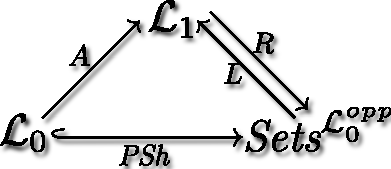
\includegraphics[width=0.5\columnwidth]{fig/ascent.pdf}
\caption{A framework for the construction of a mechanism of local-global translation of biological information. $\mathcal{L}_0$ and $\mathcal{L}_1$ are respectively the categories of relatively local and global biological information structures. The Yoneda embedding functor $PSh$ constructs the presheaf functor category on $\mathcal{L}_0$. The functors $A$, $R$, and $L$ are initially defined abstractly and subsequently constructed.}
\label{fig:ascent}
\end{figure}
\end{frame}

\begin{frame}
In order to construct the functor $L$, we need to explain the relationship between objects in the category of presheaves and the representable functors from their underlying category.
\end{frame}

\begin{frame}
\iftoggle{thmsty}{
\begin{definition}
\label{definition-category-of-elements}
}{}
For any category $\mathcal{C}$, index category $J$, and functor $A:J \rightarrow \cC$, every $P \in \Ob(\textit{Sets}^{\cC^{opp}})$ is a colimit of $\cC$-representable functors
$$
\lim\limits_{\overrightarrow{j \in J}} PSh A_j \cong P.
$$
There is a canonical choice for $J$ and $A$ such that
$$
\lim\limits_{\rightarrow{J}} PSh \circ A \cong P.
$$
The unique index category $J$ is called the {\it category of elements} of the presheaf $P$ and is denoted
$$
\int_{\cC} P.
$$
\end{frame}

\begin{frame}
The objects of $\int_{\cC} P$ are pairs $(C,x)$ where $C \in \Ob(\cC)$ and $x \in PC$. The morphisms are triples $(g,(C',x'),(C,x))$ where $g:(C',x') \rightarrow (C,x)$ derives from $g: C' \rightarrow C \in \Mor(\cC)$ and these satisfy the condition
$$
P(g)(x)=x'.
$$
There is also a projection functor that recovers structure in $\cC$ from the category of elements of $P$
$$
\pi : \int_{\cC} P \rightarrow \cC
$$
defined on objects and morphisms of the category of elements of $P$ respectively as $\pi(C,x)=C$ and $\pi (g,(C',x'),(C,x)) = g$.
\iftoggle{thmsty}{
\end{definition}
}
\end{frame}

\begin{frame}
The category of elements of a presheaf functor is depicted schematically in the figure. Colimits over the category of elements of a presheaf are used in the construction of the functors $R$ and $L$.
\begin{figure}
\noindent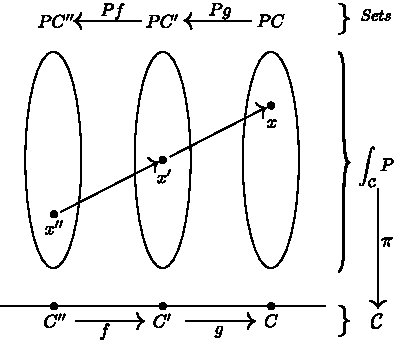
\includegraphics[width=0.6\framewidth]{fig/catofel.pdf}
\caption{The category of elements of a presheaf functor. Adapted from Awodey2006.}
\label{fig:catofel}
\end{figure}
\end{frame}

\subsection{cocompletion}
\begin{frame}
\iftoggle{thmsty}{
\begin{theorem}
\label{theorem-cocompletion-adjunction}
}{}
Consider $\mathcal{L}_0$ a small category, $\mathcal{L}_1$ is a cocomplete category, and a functor $A : \mathcal{L}_0 \rightarrow \mathcal{L}_1$. Then we can construct a pair of adjoint functors $L \dashv R$ between $\mathcal{L}_1$ and $\textit{Sets}^{\mathcal{L}_0^{opp}}$ such that $L: \textit{Sets}^{\mathcal{L}_0^{opp}} \leftrightarrows \mathcal{L}_1 :R$ where $L$ and $R$ are defined componentwise as
\begin{eqnarray}
R(L_1) &:& L_0 \mapsto Mor_{\mathcal{L}_1}(A(L_0),L_1),\\
L(P) &=& \lim\limits_{\longrightarrow} \left( \int P \xrightarrow{\pi_P} \mathcal{L}_0 \xrightarrow{A} \mathcal{L}_1 \right) .
\end{eqnarray}
\iftoggle{thmsty}{
\end{theorem}
}
\end{frame}

\begin{frame}
\iftoggle{thmsty}{
\begin{proof}
\label{proof-cocompletion-adjunction}
}{}
A natural transformation can be constructed $\tau : P \rightarrow R(L_1)$ by defining it on components as set functions parameterized by $L_0 \in \Ob(\mathcal{L}_0)$
$$
\tau_{L_0} : P(L_0) \rightarrow Mor_{\mathcal{L}_1}(A(L_0),L_1)
$$
\end{frame}

\begin{frame}
which is natural in $C$ according to the commutativity of the diagram
$$
\xymatrix{
P(L_0) \ar[r]^-{\tau_{L_0}} \ar[d]_{P(u)} & Mor_{\mathcal{L}_1}(A(L_0),L_1) \ar[d]^{A(u)^*} \\
P(L'_0) \ar[r]^-{\tau_{L'_0}} & Mor_{\mathcal{L}_1}(A(L'_0),L_1) }
$$
for all $u:L'_0 \rightarrow L_0 \in \Mor(\mathcal{L}_0)$. $\tau$ is also determined by a family of morphisms in $\Mor(\mathcal{L}_1)$ by
$$
\{ \tau_{L_0}(x):A(L_0) \rightarrow L_1 \}_{(L_0,x)}
$$
indexed by objects $(L_0,x)$ of the category of elements $\int P$. This construction is natural in objects $(L_0,x)$ in the sense that the diagram
\end{frame}

\begin{frame}
$$
\xymatrix{
A(L_0) \ar@{=}[r] \ar[dd]_{A(u)} & A\pi(L_0,x) \ar[rd]^{\tau_{L_0}(x)} \ar[dd]^{u_*} & \\
& & L_1 \\
A(L'_0) \ar@{=}[r] & A\pi(L'_0,x') \ar[ru]_{\tau_{L'_0}(x')} &
}
$$
commutes for each morphism $u$. There is thus a bijection
$$
Nat(P,R(L_1)) \cong Mor_{L_1}(LP,L_1),
$$
which is natural in both $P$ and $L_1$ demonstrating the adjoint relationship $L \dashv R$.
\end{frame}

\begin{frame}
The functor $L$ is unique for a given $A$ and all functors $A$ from a small category $\mathcal{L}_0$ to a cocomplete category $\mathcal{L}_1$ factor through the Yoneda embedding $PSh$. The Yoneda embedding is thus the universal method of appending colimits to a small category as suggested by the diagram
$$
\xymatrix{
& \mathcal{L}_1 & \\
\mathcal{L}_0 \ar[ru]^{A} \ar[rr]_{PSh} & & \textit{Sets}^{\mathcal{L}_0^{opp}} \ar@{-->}[lu]_{L}
}
$$
which commutes uniquely in $L$ for a given $A$.
\iftoggle{thmsty}{
\end{proof}
}
\end{frame}

%\begin{figure}
%\noindent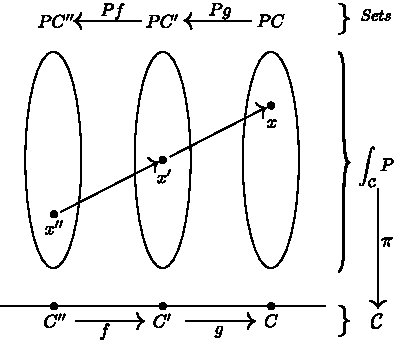
\includegraphics[width=0.8\columnwidth]{fig/catofel.pdf}
%\caption{The category of elements of a presheaf functor. Adapted from \cite{Awodey2006}.}
%\label{fig:catofel}
%\end{figure}